% 
% Licensed to the Apache Software Foundation (ASF) under one
% or more contributor license agreements.  See the NOTICE file
% distributed with this work for additional information
% regarding copyright ownership.  The ASF licenses this file
% to you under the Apache License, Version 2.0 (the
% "License"); you may not use this file except in compliance
% with the License.  You may obtain a copy of the License at
% 
%   http://www.apache.org/licenses/LICENSE-2.0
% 
% Unless required by applicable law or agreed to in writing,
% software distributed under the License is distributed on an
% "AS IS" BASIS, WITHOUT WARRANTIES OR CONDITIONS OF ANY
% KIND, either express or implied.  See the License for the
% specific language governing permissions and limitations
% under the License.
% 

    \section{Visualization}
    \label{sec:ws.vizualization}
       This page shows a visualization of all scheduled work.  Every host is represented by a square
       whose area is proportional to the amount of memory on the host.  If work is scheduled to a
       host, it is represented by a rectangle whose area is proportional to the amount of memory
       that is scheduled for the work.  In a multi-user environment, each userid is mapped into 
       a different color, making it possible to see the usage per-user.

       Hovers are provided to show the real memory size of each host, the schedulable memory for
       each host, and the amount of memory scheduled for each bit of work.

       If multiple allocations are made on a single host for the same job or service, the rectangles
       are combined into a single rectangle, reducing clutter and better showing the actual usage
       of the job (or service).   

       Clicking on any box representing scheduled work sends the browser to the details page for 
       the corresponding work.

       The screenshot below shows a visualization with a handful of 127GB hosts, 48GB hosts, and
       32GB hosts.  Regular UIMA-AS jobs show as untextured boxes; for example, job 6080, owned
       by user Hilaria, running in a 37GB allocation in host bluej291-41 which is a 127GB host.

       Hosts bluej291-45 and 291-46 are running Managed Reservations, which are shown with
       crosshatches from lower-left to upper right.

       Hosts bluej291-37 and bluej291-40 are running Unmanaged Reservations, shown with
       vertical-horizontal crosshatches.

       Below bluej291-34, bluej291-36, bluej293-49, and bluej293-60 are running {\DUCC}-managed
       services, shown by crosshatching from upper-left to lower-right.

       The host representations may be sorted by clicking on the ``size'' or the ``name'' text
       near the top of the display.


           \begin{figure}[ht!]
    \centering
    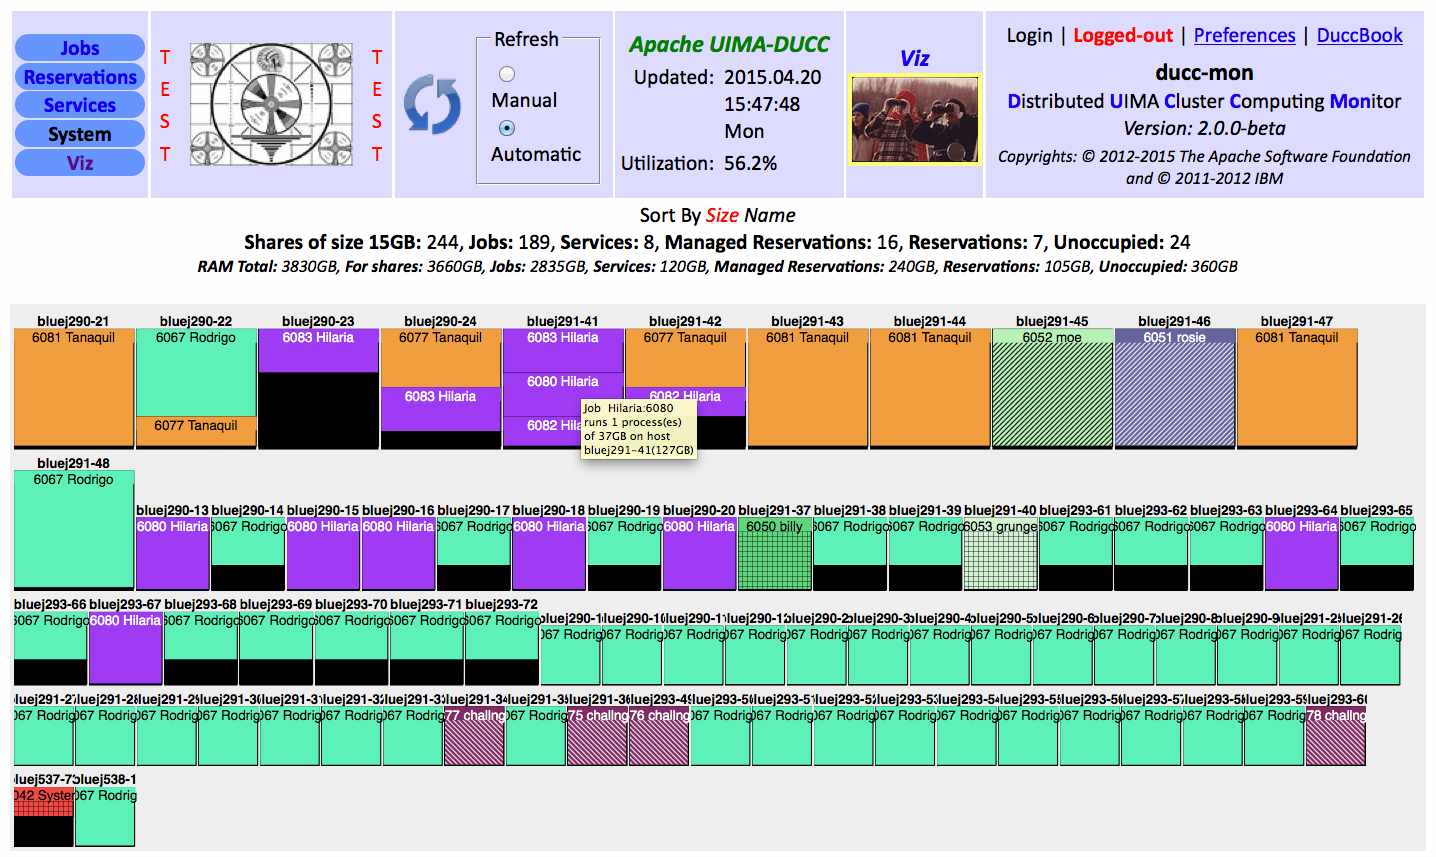
\includegraphics[width=160mm]{images/ducc-webserver/viz.jpg}
    \caption{Visualization}
    \end{figure}

